\chapter{Real-time analysis tools for the LCLS}
\label{xap}

A significant drawback of current XFELs, compared to synchrotron light sources, is that they are capable of providing photons to only one endstation at a time. As a result they are vastly oversubscribed, and beamtime is granted in small allocations through highly competitive selection processes. Experimental teams therefore have strong incentives to make the most efficient possible use of beam time. Focusing on the specific case of the LCLS, the high power of the XFEL source (and its 120 Hz repetition rate) facilitates rapid completion of experiments by making very high data collection rates possible . However, fully taking advantage of high data throughput is a problem unto itself, as experiments cannot be fully scripted in advance; it is in practice necessary to make rapid evaluations based on measurement of beam conditions (which, in two-color mode, can be strongly variable), the statistical quality of incoming data, and tentative physical interpretations in the incoming data. This feedback often guides important decisions, such as beam tuning and the motion of samples and detectors. 

With the goal of addressing this problem we have developed a software package for real-time analysis and visualization of data in XFEL experiments at the LCLS. The software is implemented using Photon Science Analysis (psana), the internal data analysis framework at the LCLS, and can be run in distributed fashion over hundreds of cores. \cite{damiani2016linac} It attempts to enable a more effective analysis workflow than currently available to LCLS users, excluding those doing specialized experiments of with well-established protocols for which there already exist tailored software packages (such as Cheetah for serial femtosecond crystallography). \cite{barty2014cheetah}

This chapter describes a Python API that that provides high-level analysis and visualization functions that directly implement common analysis operations, and can serve as a building block for creating more complex custom ones. The API is optimized for use through Jupyter Notebook, and it leverages the rich interactive plotting features available in that environment.

Though it will not be discussed in detail, we note the existence of a second interface to the same analysis framework, consisting of a web application that provides a more user-friendly graphical interface (in exchange for reduced flexibility). This interface was independently developed by Ryan Valenza from the Seidler group.



\section{Integration of Logging and Analysis}
The psana API associates every LCLS pulse (referred to as an event) with two integers, a run number and event number. \cite{damiani2016linac} A run contains a consecutive sequence of events; the maximum number of events in a run is determined by a 17 bit 360 Hz `fiducial' counter that the LCLS timing system distributes to each detector. The association of run/event number combinations to LCLS pulses is in practice further constrained by endstation-specific software and instrumental details: for example, experimental modes that require interruptions in data collections require the run number to be frequently incremented. 

Because the LCLS DAQ system does not allow the association of events with user-provided metadata, LCLS users must maintain separate experimental logs in which, for each run number and range of event numbers, they record information related to sample type, beam conditions, and other relevant experimental parameters.  In the vast majority of cases, users' analysis scripts directly expose psana's data access API, requiring them to explicitly specify datasets in terms of lists of run numbers. To do this the user must manually look up and transcribe information from the experimental logbook, an operation that becomes time-consuming (and potentially error-prone) when frequently repeated, as it usually must be.

% TODO: words
\begin{figure}[h] \label{uwxap_block}
\caption{Diagram summarizing the analysis software's architecture.}
\centering
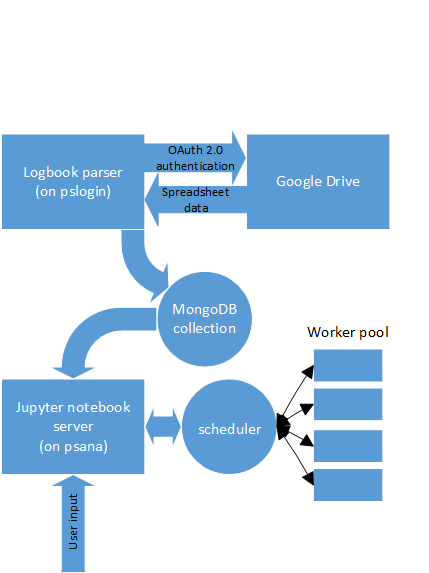
\includegraphics[scale=0.90]{../Figures/UWXAP_block_diagram.png}
\end{figure}

In response, we've made a step to unify the workflows for experimental logging and analysis. We've defined a simple query language with which the user can construct datasets defined by matches to metadata attributes recorded in the experimental logbook. The implementation is described in Fig. \ref{uwxap_block}; briefly, it consists of a daemon (i.e. application component) that accesses data from standard-formatted Google Drive spreadsheets tied to users' personal Google accounts. This daemon parses spreadsheet data into a graph structure associating run numbers with metadata column values and constructs datasets (i.e., sets of run numbers) corresponding to user-provided queries on those column values. Our Python analysis API in turn provides high-level analysis and visualization functions that operate on these user-defined datasets.

\section{Interactive Distributed Computing}
A second feature of the software is the simplified fashion in which it leverages the LCLS computing cluster. To do real-time analysis during beam runs it is typically necessary to scale one's workload over tens or hundreds of CPU cores. This is typically done with a batch processing workflow, where command lines for launching parallel analysis scripts are submitted to the LCLS's Platform Load Sharing Facility (LSF), which schedules them for execution on nodes of the cluster. Once a batch job is complete, users typically run a second (non-distributed) program to load and visualize the output data. The time that elapses between submission of a batch job and when it begins running is typically on the order 10 seconds or more, assuming an empty job queue. The separation between the steps of submitting an analysis batch job and loading and viewing its results introduces a delay as well, because the user must manually intervene at two points in the analysis pipeline. These two factors give a batch-processing-based workflow significant overhead. 

Our software package offers a significant improvement in this respect: the backend of the analysis API distributes calculations over the LCLS cluster transparently, with no need for the user to submit batch jobs or otherwise steer the parallel computation in any way. Distributed computation is implemented using the parallel computing utility pathos, which allows scatter-gather style computation using the same API as Python's multiprocessing module, but with more flexible serialization capability implemented by the module dill. 


\begin{figure}[h] \label{uwxap_screenshot}
\caption{Jupyter Notebook screen capture demonstrating a simple example of the API's usage. First a dataset is defined via a query matching all run numbers between 200 and 210 for which the recorded value for the XFEL transmission is 0.11. Two metadata attributes of the resulting dataset are then printed. In the last line of input, we call the API function datashow.show, which takes a list of datasets (in this case containing the single defined dataset) and an area detector identifier (in this case `si', the identifier for a downstream silicon spectrometer monitoring the XFEL spectrum) and displays the average of detector readouts over all events. This data was collected at LCLS beam run LK20. }
\centering
\includegraphics[scale=0.80]{../Figures/UWXAP_si_screenshot.png}
\end{figure}

\section{API features}
The last component of our package is a library of API functions for analyzing and visualizing data. These are in part tailored to MEC, the location of both our LCLS beam runs, but are for the most part generally applicable to other endstations. The API heavily leverages features of the browser-based Jupyter notebook, including interactive Javascript-based plots.


The API provides standard analysis routines for spectroscopy and X-ray powder diffraction. Miscellaneous diagnostic tools are included for, e.g., viewing the readout of area detectors (per-event or averaged over all events in a dataset) and generating histograms or scatter plots of event-by-event signal incident on arbitrary detectors. Most of these functions adopt a general functional programming style that allows the user to alter their behavior, using them as building blocks in more complex, customized applications. For instance, all analysis API calls accept, as optional arguments, user-defined functions for event rejection that take a detector datum as input and return a boolean. A more specialized example of the functions-as-arguments pattern is the histogram API call. In its most basic usage, this function takes an area detector identifier and one or more datasets as arguments, and returns an interactive figure containing histograms of per-event integrated signal on the detector. In a more sophisticated usage, the user could pass in a keyword parameter consisting of a function that, for example, integrates signal over a subregion of the area detector's 2D data array, instead of its entirety. 

This software is under continued development. The primary ongoing effort is an overhaul of the parallel-processing backend to use the distributed computing library Dask. Dask's valuable features, in our context, include a task scheduler with the ability to dispatch work to a pool of worker processes in intelligent fashion (with awareness of task dependencies and data locality), and with flexibility and fault tolerance--allowing, for example, the dynamic addition and removal of worker processes. 

